\documentclass[a4paper,12pt]{article}   % papír A4, písmo 12 bodu
\usepackage[utf8x]{inputenc}            %kodovaní UTF-8
\usepackage{ucs}                        %kodovani unicode
\usepackage[czech]{babel}               %podpora cestiny
\usepackage[T1]{fontenc}                %pouzij variantu pisma T1 (hacky, carky)
\usepackage[left=2.5cm,right=1.5cm,top=2.5cm,bottom=2.5cm]{geometry} %okraje stranky
\usepackage{amsmath,amsfonts,amssymb}   %podpora matematiky
\usepackage{gensymb,marvosym}           %symboly celsius (\celsius) apod.
\usepackage{mathptmx}                   %font Times New Roman s~podporou matematiky
\usepackage{times}                      %font Times New Roman (matematika pismem Computer Modern) 
\usepackage{parskip}                    %mezera mezi odstavci
\usepackage[none]{hyphenat} \sloppy     %slova nedelit a~nepretekat
\usepackage{titlesec}
\setcounter{secnumdepth}{4}
\clubpenalty 10000                      %kontrolovat sirotky
\widowpenalty 10000                     %kontrolovat vdovy
\usepackage{setspace} \onehalfspacing   %podpora pro zmenu radkovani + radkovani 1,5
\usepackage{enumerate}                  %podpora pro zmenu cislovani
\usepackage{fancyhdr}                   %vlastni zahlavi a~zapati
\usepackage{graphicx}                   %podpora grafiky
\graphicspath{{Materialy/}}                   %vychozi adresar s~obrazky
\usepackage{caption}                    %popisky
\usepackage{subcaption}                 %podpopisky
\usepackage{siunitx}
\usepackage{MnSymbol,wasysym}
\usepackage[shortlabels]{enumitem}
\usepackage{amsmath}
\usepackage{lastpage}                   %zjištění poslední stránky \pageref{LastPage}
\usepackage{float}                      
\usepackage{url}
\usepackage[unicode]{hyperref}          %klikaci odkazy v~textu

%----------------------------------- KONEC PREAMBULE -----------------------------------%


\newcommand{\nazev}{Měření parametrů vyšších komunikačních vrstev internetové přípojky}
\newcommand{\jmeno}{Jakub Dvořák}
\newcommand{\datum}{\today}




\begin{document} 

\setcounter{page}{0} %cislo strany
\pagestyle{empty} %stranku necislovat

%prostredi pro grafy a~schemata \begin{graf} \begin{schema}
\newfloat{schema}{htbp}{schema}\floatname{schema}{Schéma}
\newfloat{graf}{htbp}{graf}\floatname{graf}{Graf}






\begin{titlepage}
    \begin{center}
        \vspace*{1cm}
            
        \Huge
        \textbf{\nazev}
            
        \vspace{0.5cm}
        \LARGE
            
        \vspace{1.5cm}
            
        \textbf{\jmeno}
            
        \vfill
            
        \vspace{0.8cm}
            
        \Large
            
        \datum\\
        \vspace*{.5cm}
        
\includegraphics[width=.4\textwidth]{logo-cvut-fee.png}\\
    \end{center}
\end{titlepage}


% --- definice zapati a~cislovani ---
\newpage 
\pagestyle{fancy}                                       %vlastni zahlavi/zapati
\renewcommand{\headrulewidth}{0pt}                      %bez linky v~zahlavi
\renewcommand{\footrulewidth}{.5pt}                     %linka v~zapati - optional
\lhead{}       \chead{} \rhead{}                        %pole zahlavi (prazdna)
\lfoot{\nazev} \cfoot{} \rfoot{\thepage}   %pole zapati



%------------------------------------ VLASTNÍ TEXT ------------------------------------%

\subsection*{Zhodnocení naměřených hodnot}
Jak je patrné z~grafu \ref{fig:up}, uplink mé domácí přípojky je stabilní a~jen výjimečně klesá pod inzerovanou hodnotu 20~Mbit/s. Naopak downlink je mnohem nižší, než kolik udává zprostředkovatel služby. Takto výrazně nižší rychlost je dána velkou vzdáleností počítače od switche, které jsou navíc odděleny podlahou a~využíváním sítě dalšími členy domácnosti.


\begin{graf}[hbtp]
  \centering
  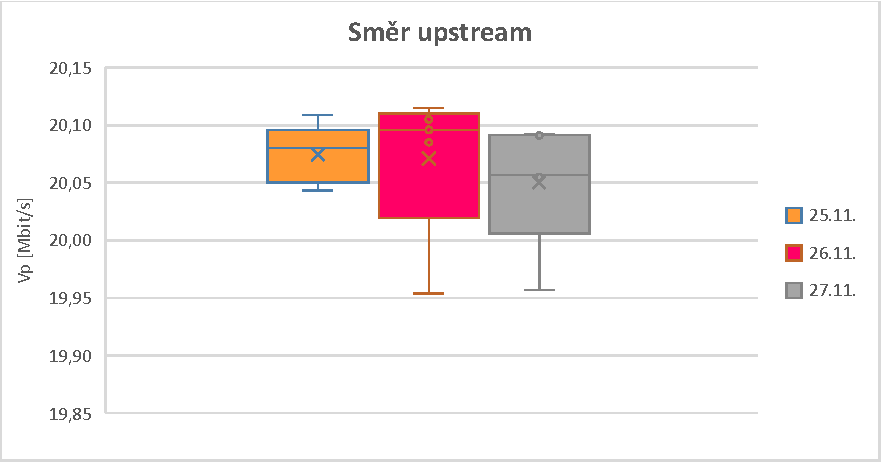
\includegraphics[width = .6\textwidth]{tsi_uplink.pdf}
  \caption{Naměřené rychlosti ve směru upstream}
  \label{fig:up}
\end{graf}

\begin{graf}[hbtp]
  \centering
  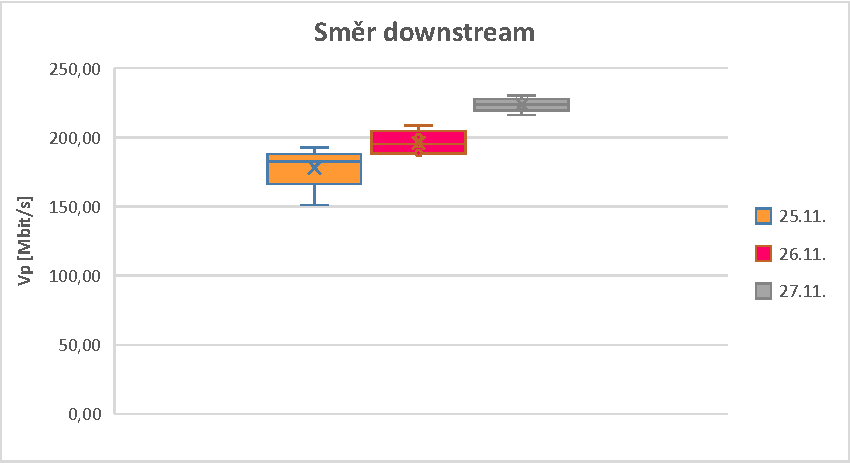
\includegraphics[width = .6\textwidth]{tsi_downlink.pdf}
  \caption{Naměřené rychlosti ve směru downstream}
  \label{fig:down}
\end{graf}


\subsection*{Podmínky měření}
Síť je tvořena centrálním modemem/routerem Compal~CH7465. Přes port 1000Base-T je připojen TP-LINK Archer~C6 nastavený jako switch. Počítač, na kterém probíhalo měření, byl připojen k~tomuto prvku přes WiFi připojení 802.11ac

Měření probíhalo na prohlížeči Google Chrome


\subsection*{Zhodnocení vhodnosti internetové přípojky pro NGA a~zařazení do příslušné NGA kategorie}
Síť je stabilní a~v~zásadě omezena primárně vzdáleností switche od měřicího počítače. Rychlost internetové přípojky ve směru downstream je tedy dostatečná a~splňuje parametry přípojky NGA~30+. Stále se bohužel jedná o~velice nesymetrický tarif, kde je rychlost odesílání dat více než desetkrát nižší jak rychlost stahování. Podle Pokynů~EU tedy přípojka resp. tarif nesplňuje požadavek NGA~100+ na rychlost ve vzestupném směru, která by měla být minimálně třetinová oproti rychlosti v~sestupném směru.

Přípojku lze tedy označit jako NGA


\subsection*{Zhodnocení vhodnosti použité přenosové technologie k~poskytovateli připojení pro koncept NGA}
Použitá technologie přípojky splňuje podmínku \uv{přístupové sítě z~optických vláken (FTTx)}

\subsection*{Kontrolní otázky}

\subsubsection*{Proč o~kvalitě internetové přípojky a~obecněji i o~poskytované přenosové službě, má pro koncového uživatele větší vypovídající hodnotu běžně dostupná rychlost, než rychlost poskytnutá diagnostikou síťového prvku.}
Jedná se o~parametr přenosové rychlosti, jak se jeví koncovému uživateli. Je v~ní zahrnuta jak výkonnost přípojky, tak výkonnost komunikační sítě poskytovatele.

\subsubsection*{Nabízí Váš poskytovatel tarif/typ připojení, které by mohlo splňovat podmínky přípojek NGA 100+? Pokud to lze dohledat, uveďte neakční cenu a~technologii.}
Pevný internet 30~Mbps~-~449~Kč\footnote{\url{https://www.vodafone.cz/_sys_/FileStorage/download/1/794/prehled-tarifu-a-sluzeb.pdf}}
\end{document}